%
\section{Motion detection}
\label{sec:motion-detection}
The \texttt{\gls{mdo-l}} needs to be capable of detecting a user, in order to switch between \texttt{normal mode} to \texttt{interaction mode}.
In order to do such thing, it is mandatory to have a system that detects the motion of a user that approaches to the local system \texttt{\gls{mdo-l}}.

\subsection{Different types of detection}
There are several ways to do motion detection, through different sensors, such as~\cite{sensors-list}:
%
\begin{itemize}
\item \emph{\gls{pir}}: A passive infrared sensor detects body heat (infrared energy) by looking for changes in temperatures. 
This is the most-widely-used motion sensor in home security systems~\cite{sensors-list}.

Once the PIR motion sensor warms up, it can detect heat and movement in the surrounding areas, creating a protective "grid".
If a moving object blocks too many grid zones and the infrared energy levels change rapidly, the infrared sensor triggers an alarm~\cite{sensors-list}.
%
\item \emph{\gls{mw}}: This type of sensor sends out microwave pulses and measures the reflections off of moving objects.
They cover a larger area than infrared sensors but are more expensive and vulnerable to electrical interference~\cite{sensors-list}.
%
\item \emph{Dual technology motion sensors}: Some motion sensors can combine multiple detection methods in an attempt to reduce false alarms.
For example, it's not uncommon for a dual technology sensor to combine a \gls{pir} sensor with a \gls{mw} sensor~\cite{sensors-list}.
%
\item Less common types of motion detectors:
	\begin{item-c}
	\item \emph{Area reflective sensors}: This kind of sensors emit infrared rays from an LED and use the reflection of those rays to measure the distance to the person or object, allowing for detection when the subject moves within the designated area~\cite{sensors-list}.
	%
	\item \emph{Ultrasonic motion sensors}: This sensors measure the reflections off of moving objects via pulses of ultrasonic waves~\cite{sensors-list}.
	%	
	\item \emph{Vibration motion sensors}: This type of sensors detect small vibrations that people cause when they move through a room~\cite{sensors-list}.
	\end{item-c}
	%
\item Specialized motion sensors:
	\begin{item-c}
	\item \emph{Contact sensors}: Contact sensors use a magnet to spot movement on a door or window. When the sensor and corresponding magnet move apart as a door or window opens, the sensor triggers~\cite{sensors-list}.
	%
	\item \emph{Pet-immune motion sensors}: Most passive infrared sensors can ignore animals up to a certain weight. A dual technology motion sensor is more pet resistant to false alarms because it requires two sensors to be triggered a certain way~\cite{sensors-list}. 
	%	
	\end{item-c}
\end{itemize}

\subsection{Trade-off between sensors}
As it can be seen previously, there are several types of sensors that can be used. However, it is mandatory to make a trade-off between each type in order to choose the better case, according several factors such as price, range, applicability, conditions of use and others.

For this specific case, it is necessary a set of sensors with a low range detection (more or less than 1,5 meters), a good reflection and low consumption. Thus, the type of sensors that match all these criteria are ultrasonic sensors.
The reasons to discard the others sensors are simple:

Firstly, the \gls{pir} sensor actuates with changes in radiation, which means that some other case can occur where is not a human approaching the \gls{mdo-l} like, for example, an animal.

In second place, the Infrared Reflective sensors have too specific characteristics of behavior. 
For example, there are some surfaces that do not reflect quite good the \gls{ir} radiation, which could easily result on a bad behavior for two different users.

Lastly, the contact sensors are out of question for obvious reasons: there is no need to have a contact between the \gls{mdo-l} and an user.

Concluding, the best option is to use a set of ultrasonic sensors, in order to avoid some specific situations and make the user detection as better as possible.

\subsection{Ultrasonic sensor}
Ultrasonic sensors work by sending out a sound wave at a frequency above the range of human hearing.
Ultrasonic waves are sound waves emitted at a frequency higher than can be detected by human hearing — typically above 20 kHz~\cite{ultrasonic-sensor-img}.

As it can be seen in Fig.~\ref{fig:ultrasonic-sensor}, many ultrasonic sensors use a single transducer to send a pulse and to receive the echo, others use one transducer to send the pulse and another to receive it.  
The sensor determines the distance to a target by measuring time lapses between the sending and receiving of the ultrasonic pulse~\cite{ultrasonic-sensor}.

\begin{figure}[!hbt]
\centering
    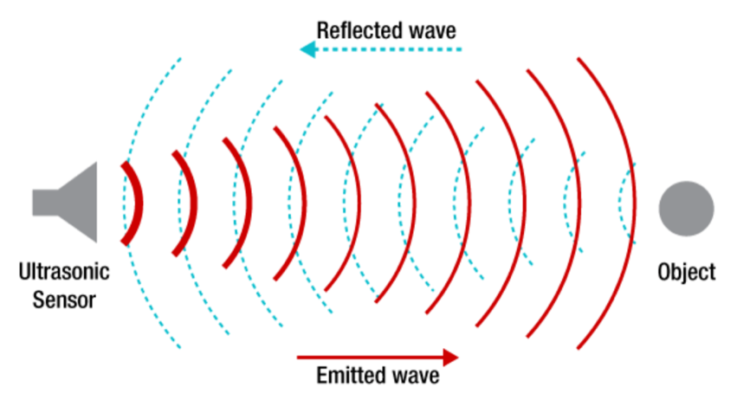
\includegraphics[width=0.6\textwidth]{./img/ultrasonic-sensor.png}
  \caption{Example of the behaviour of an ultrasonic sensor(withdrawn from~\cite{ultrasonic-sensor-img})}%
\label{fig:ultrasonic-sensor}
\end{figure}

%%% Local Variables:
%%% mode: latex
%%% TeX-master: "../../../dissertation"
%%% End:
